\documentclass[10pt,a4paper]{article}
\usepackage[utf8]{inputenc}
\usepackage[portuguese]{babel}
\usepackage[T1]{fontenc}
\usepackage{amsmath}
\usepackage{amsfonts}
\usepackage{amssymb}
\usepackage{graphicx}
\usepackage{hyperref}
\usepackage{subcaption}
\usepackage{listings}

\renewcommand{\lstlistingname}{Código}

\title{Visualização de curvas e superfícies através de geodésicas}
\author{Orientadora: Asla Medeiros e Sá\\Aluno: Cristhian Grundmann}
\date{\today}

\begin{document}

\maketitle


\section*{Geodesic Tracing}
O objeto de interesse desse projeto é o \textit{geodesic tracing},
uma técnica de visualização de superfícies baseada em \textit{ray tracing}.

\begin{figure}[h!]
\centering
\begin{subfigure}{0.4\linewidth}
\fbox{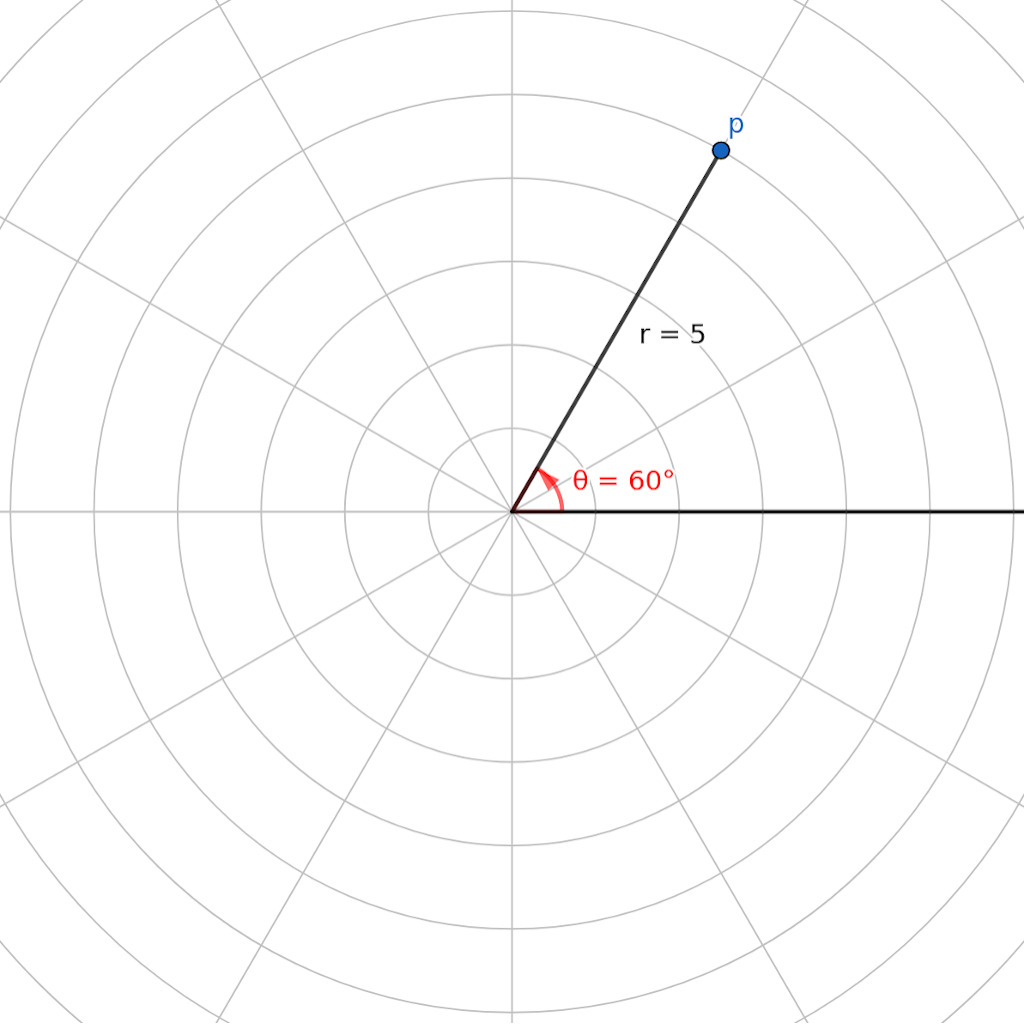
\includegraphics[width=0.9\linewidth]{polar.png}}
\caption{Plano polar - visão interna}
\end{subfigure}
\begin{subfigure}{0.4\linewidth}
\fbox{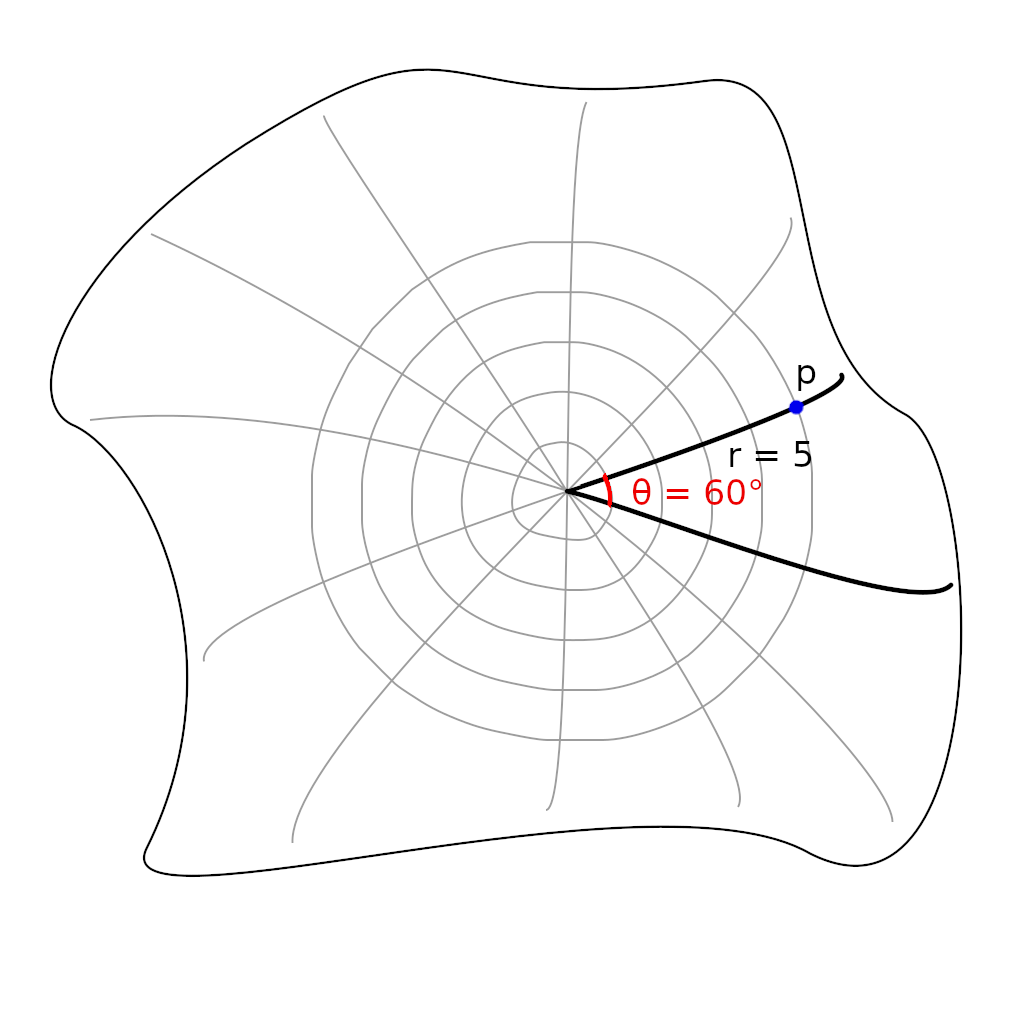
\includegraphics[width=0.9\linewidth]{geo.png}}
\caption{Superfície - visão externa}
\end{subfigure}
\caption{Geodesic tracing}
\end{figure}

Uma câmera é definida por um ponto e uma direção.
O geodesic tracing é uma aplicação do plano polar para a superfície.
A imagem do ponto $(\theta, r)$ é o ponto da geodésica de ângulo $\theta$ e de comprimento de arco $r$.
A geodésica parte da câmera e faz ângulo $\theta$ com a direção da câmera.

Para visualizar essa aplicação, é necessária uma imagem sobre a superfície.
Os pontos do plano polar são coloridos conforme a cor do ponto da sua imagem.

Uma curva geodésica em uma superfície $S$ é caracterizada pelo seguinte sistema de equações diferenciais ordinais:

\begin{align*}
\frac{d}{dt}(E\dot{u}+F\dot{v}) &= \frac{1}{2}(E_u\dot{u}^2 + 2F_u\dot{uv} + G_u\dot{v}^2)\\
\frac{d}{dt}(F\dot{u}+G\dot{v}) &= \frac{1}{2}(E_v\dot{u}^2 + 2F_v\dot{uv} + G_v\dot{v}^2)
\end{align*}

Onde $E$, $F$ e $G$ são os coeficientes da primeira forma fundamental
e $u$ e $v$ são as coordenadas da parametrização da curva.

Esse sistema geralmente não possui solução analítica ou é muito difícil de resolver.
Por esse motivo, uma solução numérica é usada no lugar. O método de Runge-Kutta pode ser uma boa escolha.

\section*{Interface gráfica e truques}
Nesse projeto, uma interface gráfica será implementada usando C++ e OpenGL.
Nela, será possível visualizar curvas e superfícies parametrizadas em 3D, além do geodesic tracing.

O usuário poderá mover a câmera do geodesic tracing e da visualização em 3D.
Além disso, poderá desenhar sobre as superfícies.
Para isso, é preciso saber os parâmetros da superfície em um ponto do desenho.
Um truque para resolver esse problema é desenhar duas vezes a superfície:

\begin{figure}[h!]
\centering
\begin{subfigure}{0.4\linewidth}
\fbox{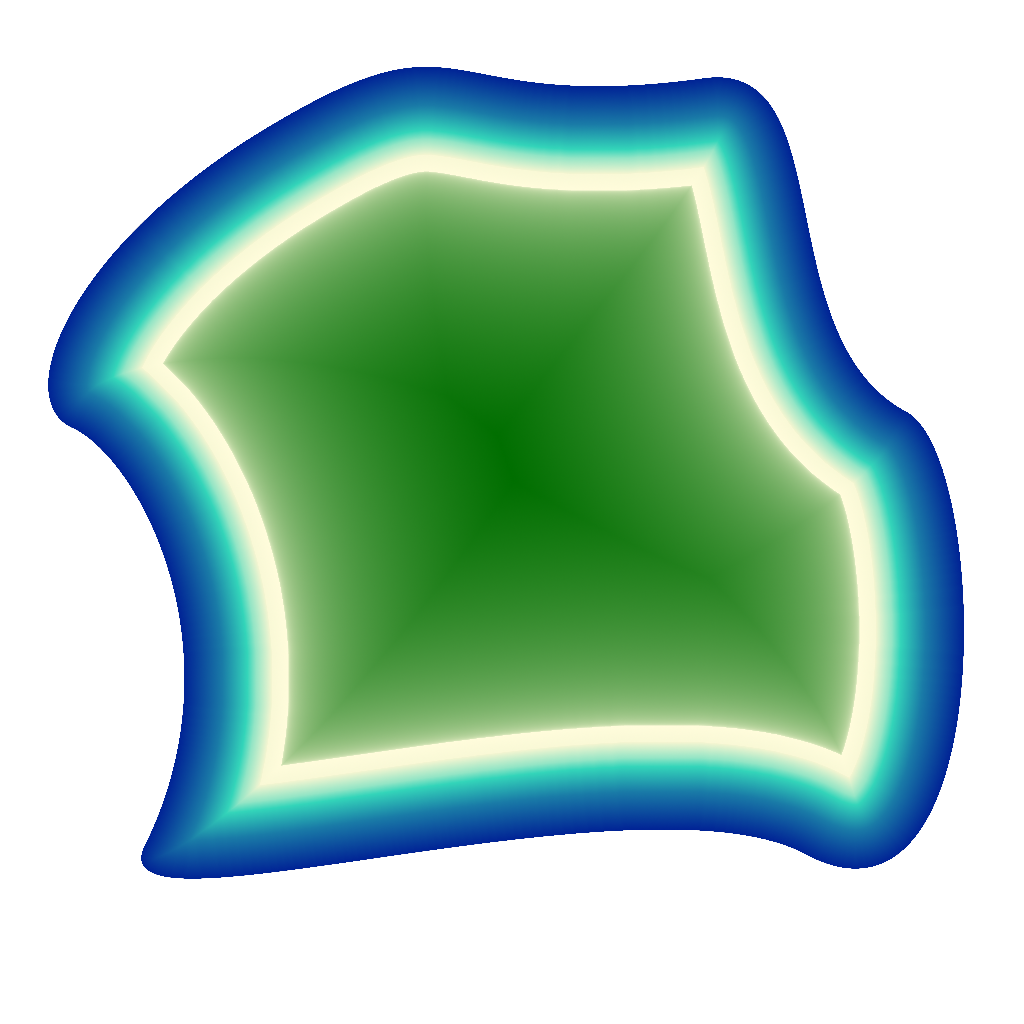
\includegraphics[width=0.9\linewidth]{img.png}}
\caption{Textura customizada - exibida}
\end{subfigure}
\begin{subfigure}{0.4\linewidth}
\fbox{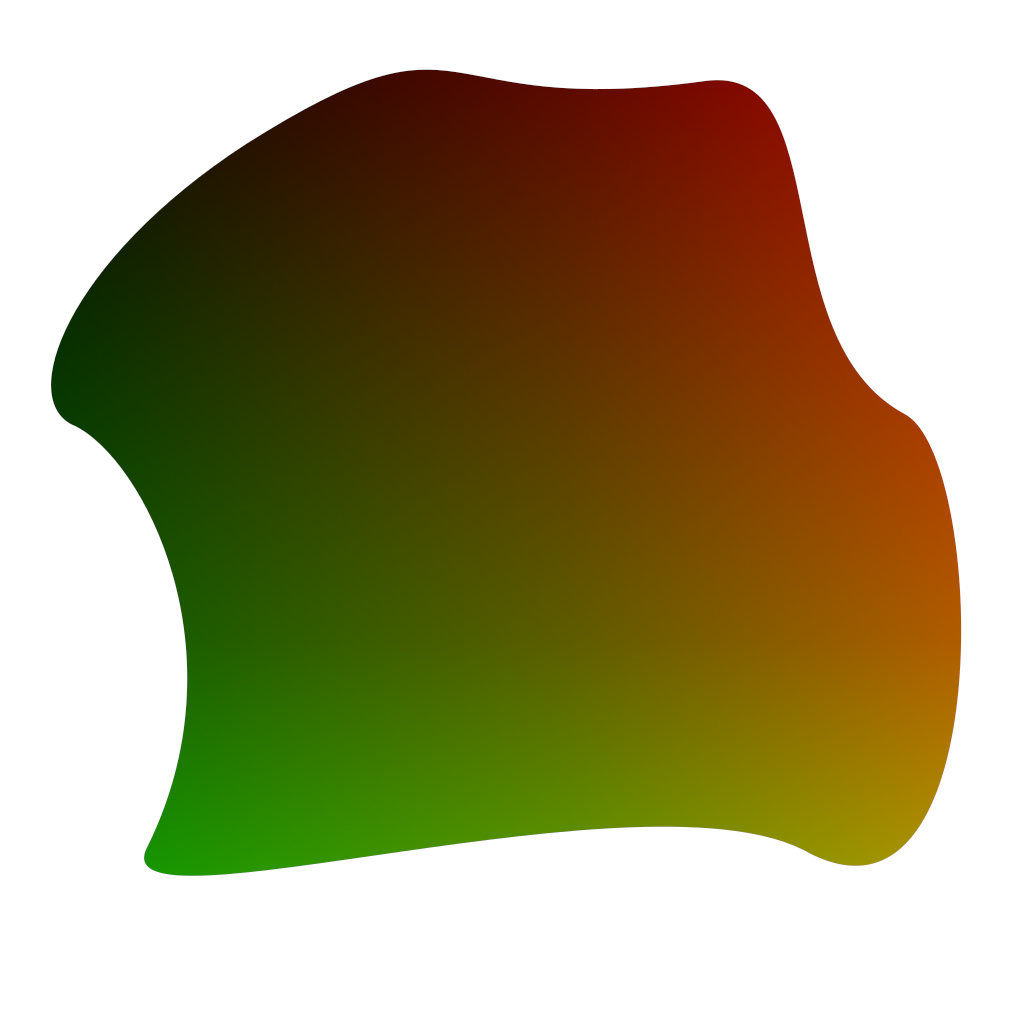
\includegraphics[width=0.9\linewidth]{uv.png}}
\caption{Textura UV - escondida}
\end{subfigure}
\caption{Truque para seleção de pontos}
\label{tracing}
\end{figure}

Assim, a cor da textura UV indica os parâmetros UV da superfície.

Outros truques de textura podem ser usados, por exemplo:

\begin{itemize}
\item Para estimar uma integral, uma textura que indica elemento de área pode ser renderizada.
Assim, para integrar uma textura qualquer, basta fazer a média das cores ponderadas pelo elemento de área.

\item Na visualização do geodesic tracing, uma textura que representa
a aplicação $(\theta, r) \rightarrow (U, V)$ pode ser renderizada.
Com essa textura é possível renderizar a imagem customizada e selecionar pontos da superfície.
\end{itemize}

\newpage
\section*{Compilação e Matemática Simbólica}

Para definir os objetos, o usuário deve fornecer uma descrição textual, que então é compilada para ser desenhada.
Por exemplo:

\begin{lstlisting}[frame=single, caption=Descrição textual]
#circle and sphere
curve	 C(t) = (cost, sint), t : [0, 2pi];
surface	 S(u,v) = (cosu, cosv sinu, sinv sinu),
	     u : [0, 2pi], v : [0, 2pi];
\end{lstlisting}

O compilador processa o texto em três etapas:

\begin{enumerate}
\item Análise léxica: detecta as `palavras' do texto, que são palavras-chave, números, funções, constantes, etc.

\item Análise sintática: detecta as estruturas do texto, resolvendo as ordem das operações, reconheçendo declarações, etc.

\item Análise semântica e síntese: verifica a validade dos objetos
e finalmente gera todas as estruturas de dados necessárias para a visualização.
\end{enumerate}

Várias derivadas parciais são exigidas para todos os fins, inclusive a equação geodésica.
Para isso, as expressões matemáticas geradas pelo compilador são derivadas simbólicamente.
Esse processo não é complexo, pois derivação é determinística e pode ser computada facilmente por recursão.

\newpage
\section*{Referências}

Pressley, A.N. (2010). Elementary Differential Geometry
(Springer Undergraduate Mathematics Series) (2nd ed. 2010 ed.).
Springer.

Wikipedia contributors. (2022, June 16). Runge-Kutta methods.
Wikipedia. https://en.wikipedia.org/wiki/Runge-Kutta\_methods

Aho, A., Lam, M., Sethi, R., \& Ullman, J. (2006). Compilers:
Principles, Techniques, and Tools (2nd ed.). Addison Wesley.

OpenGL - The Industry’s Foundation for High Performance Graphics.
(2011, July 19). The Khronos Group. https://www.khronos.org/opengl/

Learn OpenGL, extensive tutorial resource for learning Modern OpenGL.
Retrieved 2022, from https://learnopengl.com

Cornut, O. GitHub - ocornut/imgui: Dear ImGui: Bloat-free Graphical User interface
for C++ with minimal dependencies.
GitHub. Retrieved 2022, from https://github.com/ocornut/imgui



\end{document}